\documentclass[11pt]{article}
\usepackage[utf8]{inputenc}
\usepackage{graphicx}
\usepackage{titlepic}
\usepackage{caption}
\usepackage{subcaption}
\usepackage[a4paper, total={6in, 8in}]{geometry}

% \documentclass{beamer}
\usepackage{amsmath}

\newcommand{\namesigdate}[2][5cm]{%
  \begin{tabular}{@{}p{#1}@{}}
    #2 \\[0.4\normalbaselineskip] \hrule \\[0pt]
    {\small } \\[2\normalbaselineskip] 
  \end{tabular}
}

\title{\vspace*{\fill} \textbf{Automated Image Captioning}
	  \\ {\large \textbf{COD310: Mini Project}}
	  \\  \vspace{3mm} 
\includegraphics[width=5cm]{logo.jpg}}

\author{
	\textbf{Suyash Agrawal}\\ 
	2015CS10262\\
	Computer Science\\
	CGPA: 9.92 \\
	Mob: 9717060183\\
	cs1150262@iitd.ac.in
	\and
	\textbf{Madhur Singhal}\\ 
	2015CS10235\\
	Computer Science\\
	CGPA: 8.66\\
	Mob: 9540972599\\
	cs1150235@iitd.ac.in
}
\date{\textbf{Supervisor:-} \\ \textbf{Subhashis Banerjee} \\ Professor \\ Department of CSE \\ suban@cse.iitd.ac.in\\ IIT Delhi\\
\vspace*{\fill}}




\begin{document}
	\maketitle

\begin{center}
\noindent\rule{3.2cm}{0.4pt} 
\end{center}

	\newpage
	
	\section{Introduction}
	\textit{\textbf{Automated Image Description}} basically involves making a computer ``look" at an image, understand what is going on and generate a human readable description of the image. We reproduce the recent advancements in image captioning using deep neural networks, specifically an end to end image description model as described in the ``Show and Tell"\cite{showandtell} paper to achieve our goals. In simple terms the machine can interpret an image given to it because of exhaustive training over a large number of images of situations and objects common to human experience.
	
	\begin{figure}[h]
	\centering
	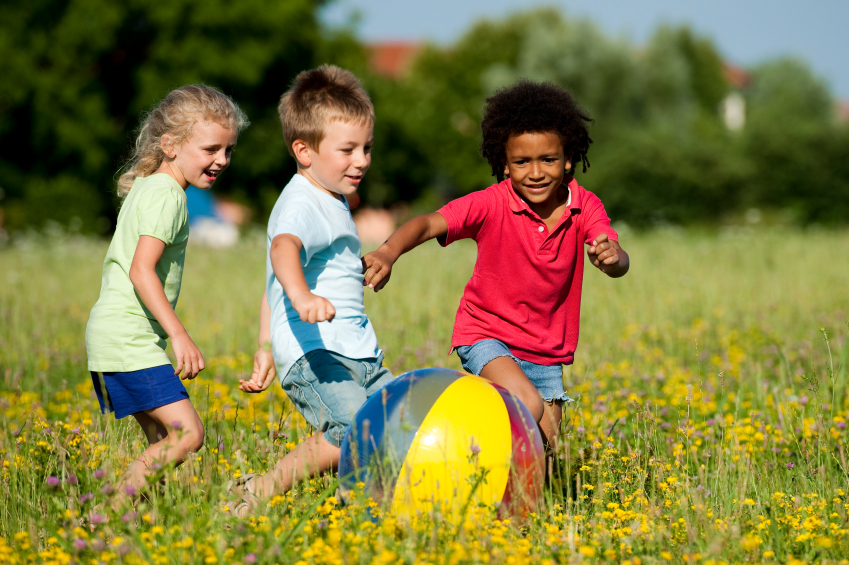
\includegraphics[width=0.5\textwidth]{children.jpeg}
	\caption{Description: A group of young children playing a game of soccer}
	\centering
	\end{figure}

	\section{Motivation}

The inspiration for this project came from our plan to do a SURA project on ``Video Description". Since image description has recently been done to a reasonable accuracy so the first step for doing video description is to understand and implement current state of the art image description / captioning techniques. Thus the primary objective of this mini project was to familiarize ourselves with Deep Learning Techniques, learn to use the libraries and to gain insight into how image captioning is performed so that we can move onto the more complicated task of video captioning .	

	\section{Methodology}
		Image captioning model basically consists of two broad models:
		\begin{enumerate}
		\item
			\textbf{Image Encoder}: A deep CNN network (Inception V3) to encode images to fixed length vector representation.
		\item
			\textbf{Sequence Decoder}: An LSTM network to decode the encoded information in form of description.
		\end{enumerate}
	
		\begin{figure}[ht!]
		\centering
		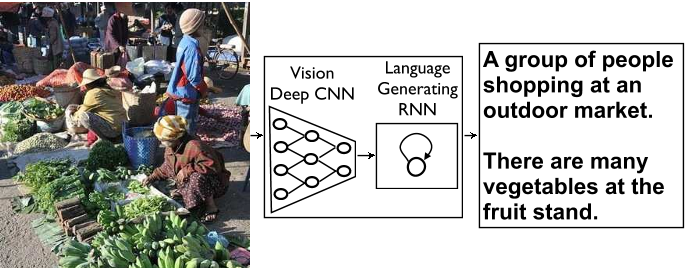
\includegraphics[width=0.8\textwidth]{model.png}
		\caption{High level representation of image captioning model}
		\centering
		\end{figure}
	
		\subsection{Image Encoder}
			Image encoder is basically a deep CNN network pretrained on image classification dataset (ImageNet). This was chosen because CNNs are state-of-art models for object recognition and as image description relies heavily on object recognition, it became an apparent choice. Also, as these were pretrained on large object classification datasets, it was certain that they are very well optimized and are able to gather high level information from images and thus are suitable for encoding images to fixed length vector.
		\subsection{Sequence Decoder}
			LSTM were used as sequence decoders. This is so because LSTM have been very successful in tackling the problem of keeping long term dependencies and deal well with problem of exploding and vanishing gradients. Basically this unit took a fixed length vector (encoded image) as input and gave out a complete sentence that represented that input.\\
			These underlying process that is followed is:
			\begin{subsubsection}{Training Process}
				\begin{enumerate}
				\item Encoded image is fed into LSTM network to inform it about the contents
				\item A special start symbol is fed into LSTM to mark the start of sentence.
				\item For each word in our dictionary, LSTM unit gives a probability of it being the first word of our predicted caption.
				\item Then first word from the correct caption is given as input to LSTM unit and LSTM outputs the probability for second word.
				\item We then recursively do this procedure until we consume our whole caption.
				\item The loss is then calculated as sum of negative log probabilities of predicting correct word at each step above.
				\end{enumerate}
			\end{subsubsection}
			\begin{subsubsection}{Inference Process}
				\begin{enumerate}
				\item Encoded image is fed into LSTM network to inform it about the contents
				\item A special start symbol is fed into LSTM to mark the start of sentence.
				\item For each word in our dictionary, LSTM unit gives a probability of it being the first word of our predicted caption.
				\item We take the word with highest probability as our first word and feed it into LSTM to get second word
				\item We then recursively do this procedure until we get special END word as output or we reach max length.
				\item The caption generated is basically just the sequence of predicted words by our LSTM.
				\end{enumerate}
			\end{subsubsection}
		\subsection{Overall Model}
			\subsubsection{Training}
				\begin{itemize}
				\item An image and caption pair is fetched from training dataset
				\item Image is fed into Image Encoder network to generate encoded vector.
				\item This vector along with correct caption is fed into Sequence Decoder network to get loss.
				\item This loss is backpropagated in neural network so that it can "learn" from process.
				\end{itemize}
			\subsubsection{Inference}
				\begin{itemize}
				\item Test image is fed into Image Encoder network to generate encoded vector.
				\item This vector fed into Sequence Decoder network which generates a set of captions.
				\item No backpropagation happens in this case as we don't know the correct caption and are just testing our network.
				\end{itemize}	
	\section{Our Work}
	
 We were new to the field of deep learning, thus this project involved a lot of independent study so that we could understand the field and follow along with literature. We referred to Stanford's CS231N \cite{cs231n} and fast.ai's Deep Learning MOOC\cite{fastai} for a thorough introduction to these techniques and their implementation. We also learned to program in Keras and Tensorflow, two widely popular deep learning libraries which are programmed using Python.  After getting a grasp of deep learning we proceeded into the image captioning part of the project. Here we first studied the ``Show and Tell" paper\cite{showandtell} thoroughly and figured out how it worked. We then took the reference code of ``Show and Tell" for Tensorflow provided by the authors and modified it to run on our computers with any provided image.\\\\Deep Learning models require ``training" before they can be used, so we downloaded the MSCOCO \cite{mscoco} dataset of 80,000 images along with their descriptions. We used a pre-trained Inception v3  model for the CNN, this is basically a 30 layer network which produces a vector encoding of an image which can be used further. The LSTM network in the model still needs to be trained so we set up the whole training process on a computer in the lab. The training process of the LSTM network with the 80k image dataset took about 2 days on one computer in the Vision Lab. Further we performed Fine-Tuning on the dataset so that the CNN layer could be appropriately adjusted. The finetune process took about 4 days on the same computer. After this we tried to use the model to caption several images locally and it performed well. we even set up a demo on Open House where people could choose images and have them described by our neural model locally. Finally, to assess how good, the whole image description stack worked we conducted a small survey where we gave a group of people some images which had been captioned by the model and asked them to score it on the basis of accuracy and relevance. The results are presented with this report.
\newpage
	\section{Results}
		After training our model we tested it on a random batch of images to generate captions. Then we setup a small survey in which we asked people to rate the caption on the basis of relevance . We also got reasonable idea about its accuracy during our demo in Open House where we asked people to give any image as input to our model and rate the caption generated by it. Some of the sample captions generated are as follows:
	
\begin{figure}[ht!]
			    	\centering
					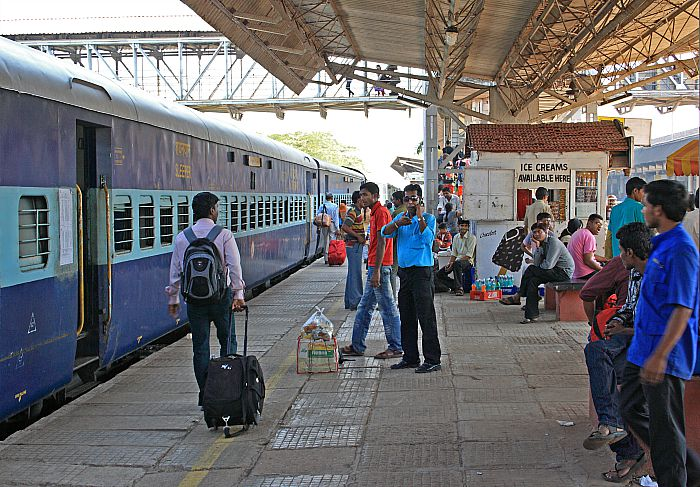
\includegraphics[scale=0.266]{margao_railwaystation_1441973309.jpg}
					\caption{A group of people standing next to a train .\label{fig11}}
\end{figure}
\begin{figure}[ht!]
			    	\centering
					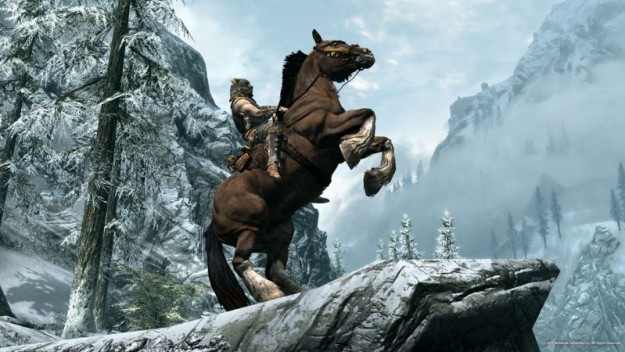
\includegraphics[scale=0.266]{skyrim_Horse01-625x352.jpg}
					\caption{A man riding a horse in the snow .\label{fig12}}
\end{figure}
	\newpage
	\section{Background} 
			\subsection{Deep Learning}
				Deep Learning is a branch of machine learning in which multiple parameter based models are used in series. In a deep network, there are many layers between the input and output, allowing the algorithm to be executed in multiple processing steps, composed of \textbf{multiple linear and non-linear transformations}. At each layer, the signal is transformed by a processing unit, like an artificial neuron, whose parameters are \textbf{`learned'} through training. Deep Learning has been shown to excel in tasks where the goal is to find \textbf{intuitive} patterns in the data.\cite{deep} In particular, in the field of Computer Vision, deep networks are increasingly used to extract \textbf{feature descriptions and inter-relationships between features} from images.\cite{cs231n}
				\begin{figure}[ht!]
					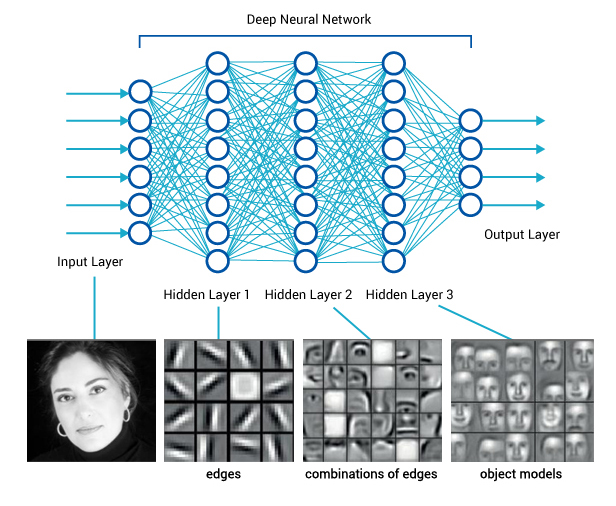
\includegraphics[width=14cm]{blog_deeplearning3.jpg}
					\caption{Illustration of Deep Learning as applied to Vision\label{fig2}}
				\end{figure}	

			\subsection{Convolutional Neural Networks}
			Convolutional Neural Networks (CNN, or ConvNet) are a type of feed-forward artificial neural network in which the connectivity pattern between the neurons is inspired by the organization of the animal visual cortex. Individual cortical neurons respond to stimuli in a restricted region of space known as the \textbf{receptive field}. The receptive fields of different neurons partially overlap such that they tile the visual field. The response of an individual neuron to stimuli within its receptive field can be approximated mathematically by a \textbf{convolution operation}. A Convolutional Neural Network consists of the following layers.\cite{showandtell}
								
				\begin{figure}[ht!]
					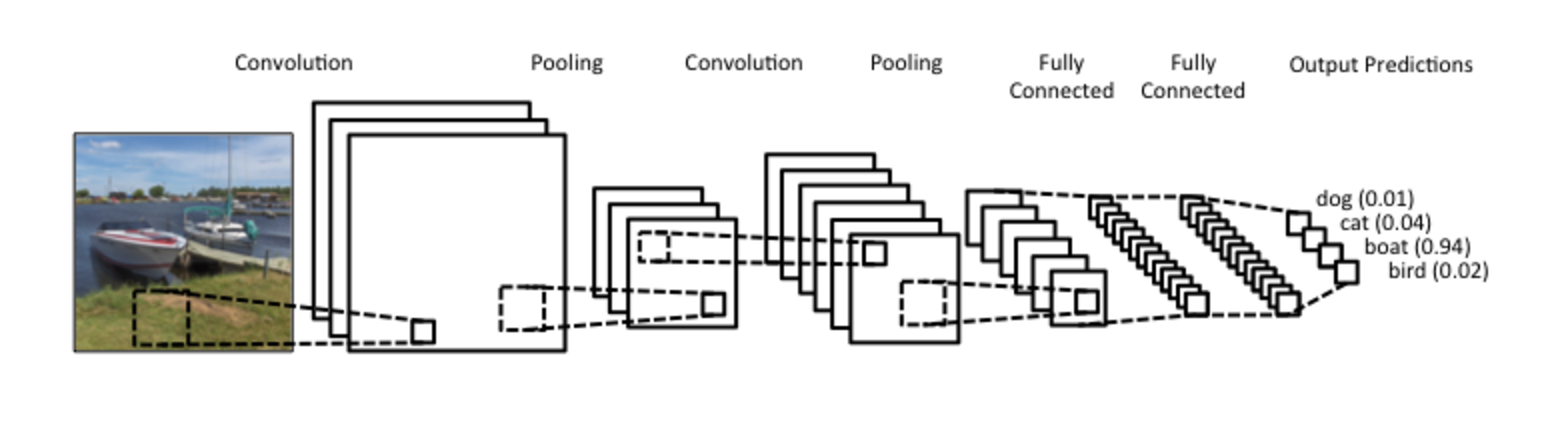
\includegraphics[width=1.0\textwidth]{conv.png}
					\caption{A Typical Convolutional Neural Network\label{fig4}}
				\end{figure}
			%skipping Relu layer since its not in picture assume it to be in conv layer
				\subsubsection{Convolutional Layer}
					The convolution layer is the core building block of a CNN. The layer's parameters consist of a set of \textbf{learnable filters} (or kernels), which have a small receptive field, but extend through the full depth of the input volume. During the forward pass, each filter is convolved across the width and height of the input volume, computing the dot product between the entries of the filter and the input and producing a $2$-dimensional activation map of that filter.\cite{cs231n} As a result, the network learns filters that activate when it detects some specific type of feature at some spatial position in the input.

				\subsubsection{Max Pooling Layer}
					It is common to periodically insert a Pooling layer in-between successive Conv layers in a ConvNet architecture. Its function is to \textbf{progressively reduce the spatial size} of the representation to reduce the amount of parameters and computation in the network, and hence to also control over-fitting. The Pooling Layer operates independently on every depth slice of the input and resizes it spatially, using the max operation.\cite{cs231n}
				\subsubsection{Fully-Connected Layer}
					Finally, after several convolutional and max pooling layers, the high-level reasoning in the neural network is done via fully connected layers. Neurons in a fully connected layer have \textbf{full connections to all activations} in the previous layer, as seen in regular Neural Networks. Their activations can hence be computed with a matrix multiplication followed by a bias offset.\cite{fullyconnected} Thus output of the fully connected layer is a vector with elements representing the `probability' (not in a strictly statistical sense) of the image containing specific objects or actions.

			\subsection{Long Short Term Memory Networks}
			    \begin{figure}[ht!]
			    	\centering
					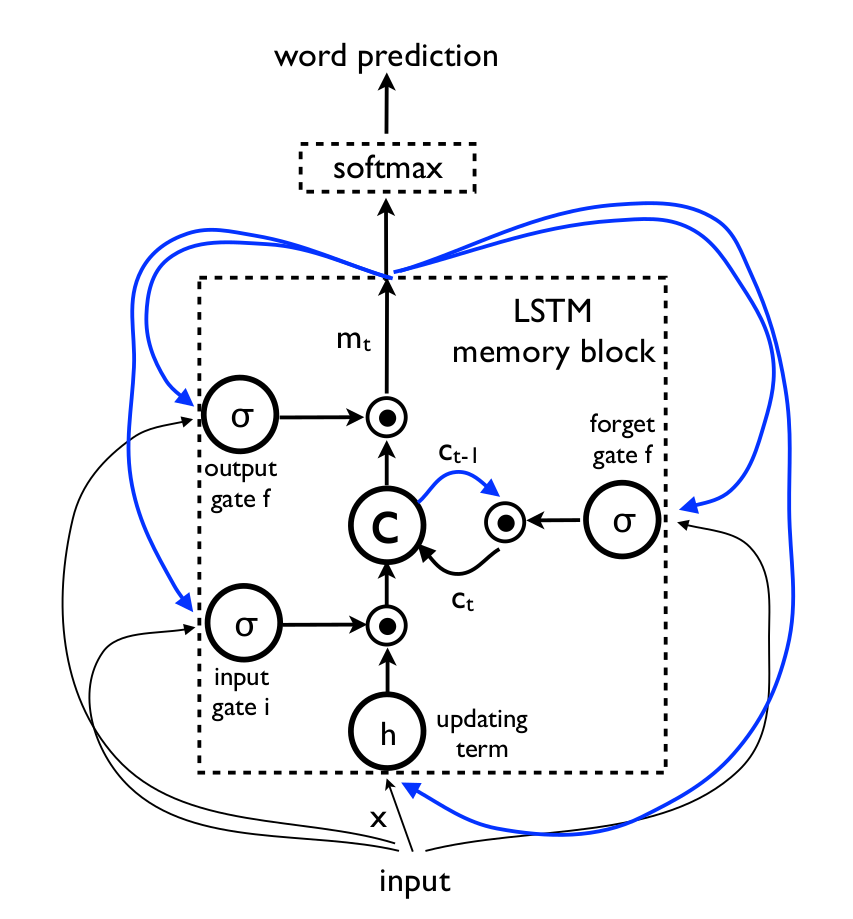
\includegraphics[scale=0.266]{LSTM_unit.png}
					\caption{A single LSTM unit\label{fig6}}
				\end{figure}
				Long Short Term Memory Networks are a type of Recurrent Neural Networks. These networks are based upon recursion, so that variable length inputs can be handled easily and sequential information can be processed with better results. LSTM's are specifically used for making RNNs learn long term patterns since traditional RNNs tend to \textbf{favour short term temporal dynamics}. It can be difficult to train traditional RNNs to learn long-term dynamics, likely due in part to the \textbf{vanishing and exploding gradients problem} that can result from propagating the gradients down through the many layers of the recurrent network, each corresponding to a particular time step\cite{ltms}. LSTMs provide a solution by incorporating memory units that explicitly allow the network to learn when to ``forget'' previous hidden states and when to update hidden states given new information\cite{lstmexecute}.\\
%				Below we list the main equations governing the behaviour of the LSTM networks.\\
%				\begin{align}
%					f_{t} &= \sigma_{g}(W_{f}x_{t} + U_{f}h_{t-1} + b_{f})\\	
%					i_{t} &= \sigma_{g}(W_{i}x_{t} + U_{i}h_{t-1} + b_{i})\\
%					o_{t} &= \sigma_{g}(W_{o}x_{t} + U_{o}h_{t-1} + b_{o})\\
%					c_{t} &= f_{t} \circ c_{t-1} + i_{t} \circ \sigma_{c}(W_{c}x_{t} + U_{c}h_{t-1} + b_{c})\\
%					h_{t} &= o_{t} \circ \sigma_{h}(c_{t})
%				\end{align}
%				The symbol meanings are:\\
%	$\mathbf{x_{t}}$: Input vector\\
%    $\mathbf{h_{t}}$: Output vector\\
%    $\mathbf{c_{t}}$: Cell state vector\\
%    $\mathbf{W}$, $\mathbf{U}$ and $\mathbf{b}$: Parameter matrices and vector\\
%    $\mathbf{f_{t}}$: Forget gate vector. Weight of remembering old information.\\
%    $\mathbf{i_{t}}$: Input gate vector. Weight of acquiring new information.\\
%    $\mathbf{o_{t}}$: Output gate vector. Output candidate\\
%    $\mathbf{\sigma_{g}}$, $\mathbf{\sigma_{c}}$ and $\mathbf{\sigma_{h}}$: Activation functions\\
		
			\subsection{Training Deep Neural Networks}
					\begin{figure}[ht!]
					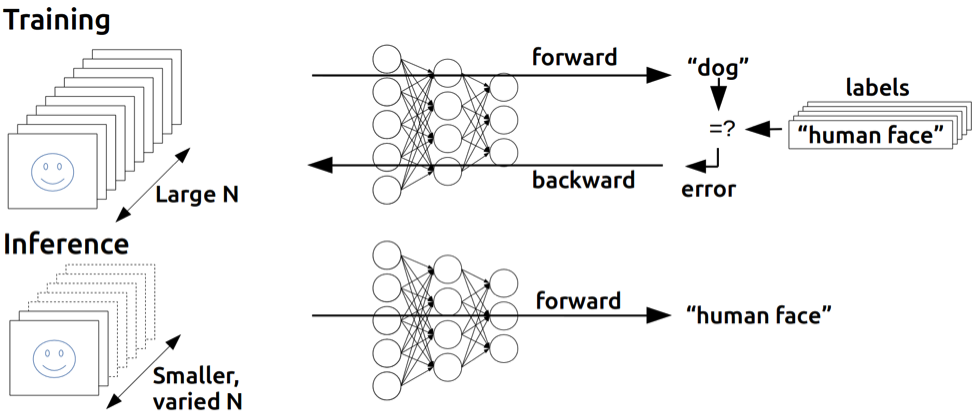
\includegraphics[width=14cm]{training_inference1.png}
					\caption{Training and Inference Processes\label{fig5}}
				\end{figure}
				A Deep Neural Network is at it's core a parameter based function. All of these parameters are  \textbf{trained} automatically from inputs and expected output tuples (training data). The training process revolves around minimizing a particular cost function using methods like \textbf{Stochastic gradient descent}. The input is given to the network in a feed forward fashion and the parameters are modified from the last layer to the first \textbf{(Backpropagation)}. Neural Networks, by design, require huge amounts of training data and take a large time to get trained. For some perspective, most current state of the art image classifiers have $> 100$ million parameters and are trained on more than 1.2 million images. 


			\subsection{Finetuning}
				Fine-tuning a network is a procedure based on the concept of
				\textbf{transfer learning}. We start training a CNN to learn features for a broad domain with a
				classification function targeted at minimizing error in that domain. Then, we
				replace the classification function and \textbf{optimize the network} again to minimize
				error in another, more specific domain. Under this setting, we are transferring
				the features and the parameters of the network from the broad domain to the
				special one.\cite{fineplant} In our project we will need to use the pre-trained image classification models 
				to actually decode individual frames of the video, thus we are planning to \textbf{fine-tune those models
				with respect to the output of our LSTMs}.



	\begin{thebibliography}{1}
	
	  \bibitem{showandtell} Oriol Vinyals and
               Alexander Toshev and
               Samy Bengio and
               Dumitru Erhan {\em Show and Tell: {A} Neural Image Caption Generator} 2014.

        \bibitem{lstmexecute} Wojciech Zaremba, Ilya Sutskever {\em Learning to Execute} ICLR 2015
         

         \bibitem{ltms} Jeff Donahue, Lisa Anne Hendricks, Marcus Rohrbach, Subhashini Venugopalan, Sergio Guadarrama, Kate Saenko, Trevor Darrell {\em Long-term Recurrent Convolutional Networks for Visual Recognition and Description} 2016

         \bibitem{deep} Bengio, Yoshua; LeCun, Yann; Hinton, Geoffrey {\em Deep Learning} 2015

         \bibitem{fineplant} Angie K. Reyes, Juan C. Caicedo and Jorge E. Camargo {\em Fine-tuning Deep Convolutional Networks for
		Plant Recognition} LifeCLEF 2015

         \bibitem{cs231n} Andrej Karpathy {\em 
			CS231n Convolutional Neural Networks for Visual Recognition
		} http://cs231n.github.io/convolutional-networks/

		\bibitem{mscoco} Tsung-Yi Lin, Genevieve Patterson et al. {\em MS COCO: Common Objects in Context
		}  http://mscoco.org/dataset

		\bibitem{fastai} Jeremy Howard {\em Practical Deep Learning For Coders, Part 1
		}  http://course.fast.ai/

		\bibitem{fullyconnected} Santanu Chaudhury, Anupama Mallik, Hiranmay Ghosh {\em Multimedia Ontology: Representation and Applications
		} 

	\end{thebibliography}
\end{document}